\chapter{Requirements}
\label{requirements}

\section{Introduction}

Requirements Elicitation is an important step in the development of a software application. There are a number of techniques possible, such as "interviewing, protocol analysis, repertory grid, work groups" \parencite{davis2006effectiveness}. Structured interviews "appear to be one of the most effective elicitation techniques in a wide range of domains and situations" \parencite{davis2006effectiveness}. 

In eliciting possible requirements for the site, there was a discussion with three club members with varying backgrounds and experience within the club.

\begin{table}[H]
\caption{Stakeholders for Requirements Elicitation}
\begin{center}
    \begin{tabular}{ | l | l | l | l | l| p{5cm} |}
    \hline
    Name & Age Bracket & Club Role & Club Membership & Work Background \\ \hline
	S1 & 35 - 45& Committee Member & 5 years & Senior Software Engineer \\ \hline
	S2 & 18 - 25 & New Member & 1 year & Graduate Software Engineer \\ \hline
	S3 & 55+ & Senior Member & 10+ years & Retired Public Servant \\ \hline
    \end{tabular}
\end{center}
\label{fig:userelicit}
\end{table}

\section{Methodology}



\section{Methods for Requirements Elicitation}

\subsection{Storyboarding}

At an early stage of the application, rough storyboards were prepared for the FYP presentation. These storyboards were used to demonstrate how a page, such as the timetable shown in Figure~\ref{fig:timetableSB}, would be displayed by the application.

\begin{figure}[H]
\begin{center}
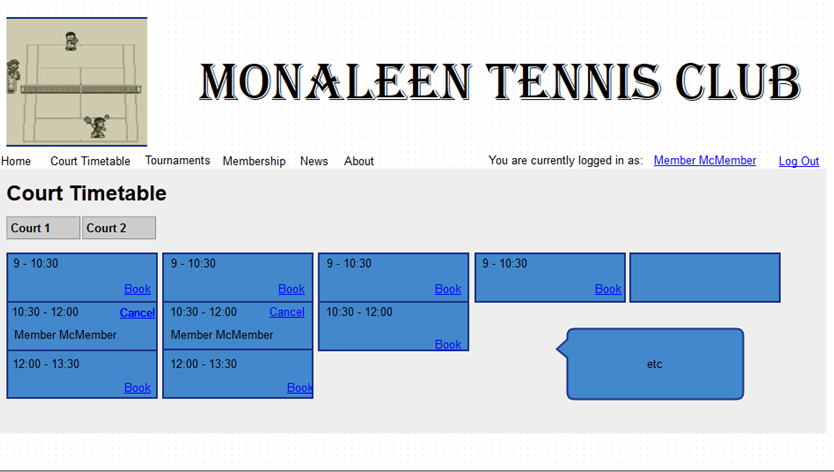
\includegraphics[width=14cm]{storyboard.png}
\end{center}
\caption{Timetable Storyboard, October 2013}
\label{fig:timetableSB}
\end{figure}

The storyboarding visualised aspects of the site, and gave a rough idea of functionality that would be needed within the application. 

\subsection{Interviews}

In order to elicit requirements, a number of interviews were held with stakeholders. These questions are listed in~\ref{sec:regquestions},~\nameref{sec:regquestions}.

During the elicitation process a number of areas were highlight as desired features.

\begin{enumerate}
\item Online Timetable
\begin{itemize}
\item Allow members to view courts and make/view bookings
\end{itemize}
\item Tournaments
\begin{itemize}
\item Allow user to register for a tournament, and view tournaments ongoing.
\end{itemize}
\item Contact Members
\begin{itemize}
\item Easy way to contact all members
\end{itemize}
\item Member Directory
\begin{itemize}
\item A list of all members, contact details, roles
\end{itemize}
\item News Section
\begin{itemize}
\item Create new items to display for members
\end{itemize}
\item Members Area
\begin{itemize}
\item A secure area that only members could access
\end{itemize}
\item Member Application
\begin{itemize}
\item Automated registration, replace old paper form
\end{itemize}
\item Club Map
\begin{itemize}
\item Directions to the club for new members and non-local visitors
\end{itemize}
\item Contact Details
\begin{itemize}
\item Information on how to contact within the club for specific needs
\end{itemize}
\item Statistics
\begin{itemize}
\item Such as games played, Win/Loss ratio
\end{itemize}
\end{enumerate}
\begin{table}[H]
\label{fig:requirementsFeatures}
\caption{Requested Features}
\end{table}
Table ~\ref{fig:reqbreakdown} refers to each numbered requirement, and whether it was brought up by a stakeholder during the elicitation process.
\begin{table}[H]
\caption{Requested Feature Breakdown}
\begin{center}
    \begin{tabular}{ | l | l | l | l| l| l| l| l| l|l| p{.22cm} |}
    \hline
     \textit{Name}& 1& 2 & 3 & 4 & 5 & 6 & 7 & 8 & 9 & 10\\ \hline
	 S1 & N & Y & Y & Y & Y & Y & Y & Y & Y & N\\ \hline
	 S2 & Y & Y & Y & N & N & N & N & N & N & Y\\ \hline
	 S3 & Y & N & N & N & N & N & Y & Y & N & N\\ \hline
  Total & 2 & 2 & 2 & 1 & 1 & 1 & 2 & 2 & 1 & 1\\ \hline
    \end{tabular}
\end{center}
\label{fig:reqbreakdown}
\end{table}

This features were broken down into four categories: \textit{Timetable}, \textit{Tournaments}, \textit{Members}, and \textit{News}.

\section{Application}

\section{Functional Requirements}

\subsection{Timetable} 

The timetable is the core aspect of the application, and one that would be most likely to be used by all members, not just those involved competitively. While the regular member would only be concerned with the booking of slots, there are a number of requirements defined for use by the administrator in order to configure a relevant timetable not the club. The timetable needs to be flexible to allow the administrator full control at all stages.

\begin{enumerate}
\item Flexible 
\item Edit individual slots
\item Define a template for a timetable
\item Reset timetable
\item Define look ahead for timetable (how many weeks in advance a user can see)
\item Delete timetable
\item Enable and disable timetable
\item Timetable analysis (No slots free, booked etc)
\end{enumerate}

\subsection{Tournament}

\subsection{News}

\subsection{Members}

\section{Use Cases}

\begin{usecase}
\addtitle{Use Case 1}{View All Members} 
\addfield{Scope:}{System-wide}
\addfield{Level:}{User can view a list of all registered, and approved, members of the club}
\addfield{Primary Actor:}{All Registered and Authenticated Users}
\additemizedfield{Stakeholders and Interests:}{
	\item All Users: contact information for club members
}

\addfield{Preconditions:}{User is registered and approved}
\addfield{Postconditions:}{User must be authenticated by the framework}
\addscenario{Main Success Scenario:}{
	\item User logs in
	\item User clicks on View Members
	\item System displays member information
}
\addscenario{Extensions:}{
	\item[1.a] Invalid login data:
		\begin{enumerate}
		\item[1.] System shows failure message
		\item[2.] User returns to step 1
		\end{enumerate}
	\item[1.a] User not approved:
		\begin{enumerate}
		\item[1.] System shows failure message
		\item[2.] Admin is emailed about attempted access by unapproved member
		\end{enumerate}
}
\addfield{Frequency of Occurrence:}{High}
\end{usecase}

\section{Non Functional Requirements}

\subsection{Security}

Since user details would be stored in the application, security of this data was highlighted as a concern. While no payment information would be held by the application, there would be names, addresses and phones numbers held within the application. The security of this information would need to be ensured.

\subsection{Extensibility}

Extensibility of the application was discussed with particular attention of the ability of the application to deal with changed to the club structure. Currently, the club has two courts in which users can book time for games. It is likely that the club will be expanding in the near future. This will result in the creation of four next courts in the near future. The application should be able to scale with this possibility without issue.

Tournaments were also mentioned as an area where future requirements may stem from. Currently, the club operates three kinds of tournaments: Singles, Doubles and Mixed Doubles. These are broken down into Ladder style tournaments and Bracket style tournaments. The club regularly holds tournaments with other national tennis clubs. The ability to create tournaments that suit these events could be necessary.

\subsection{Usability}

The age of the club members range from 8 to 80, so ease of use of any software solution is important. If a system is going to replace the existing system that all can use, a similar level of usability is required. The most common function used by members is the reservation of time slot in one of the courts. A software alternative needs to be intuitive for all members.

\subsection{Performance}

